%!TEX program = xelatex
% 完整编译: xelatex -> bibtex -> xelatex -> xelatex
\documentclass[lang=cn,11pt,a4paper,cite=authoryear]{elegantpaper}

\title{软件工程课程设计报告}
\author{毛亚琛 \\ 南京农业大学}

\date{\zhtoday}


% 本文档命令
\usepackage{array}
\newcommand{\ccr}[1]{\makecell{{\color{#1}\rule{1cm}{1cm}}}}
\graphicspath{{../../活动图/out/}{../../类图/out/}{../../设计类图/out/}{../../时序图/out/}{../../用例图/out/}}

\begin{document}

\maketitle

% \begin{abstract}
% 本文为 \href{https://github.com/ElegantLaTeX/ElegantPaper/}{ElegantPaper} 的说明文档。此模板基于 \LaTeX{} 的 article 类,专为工作论文写作而设计。设计这个模板的初衷是让作者不用关心工作论文的格式,专心写作,从而有更加舒心的写作体验。如果你有其他问题、建议或者报告 bug,可以在 \href{https://github.com/ElegantLaTeX/ElegantPaper/issues}{GitHub::ElegantPaper/issues} 留言。如果你想了解更多 Elegant\LaTeX{} 项目组设计的模板,请访问 \href{https://github.com/ElegantLaTeX/}{GitHub::ElegantLaTeX}。
% \keywords{Elegant\LaTeX{},工作论文,模板}
% \end{abstract}


\section{需求文档}

\begin{figure}[]
    \centering
    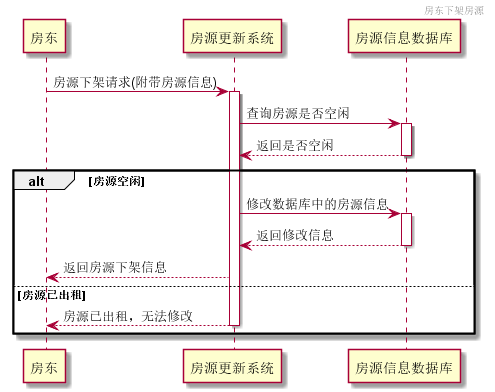
\includegraphics[width=\textwidth]{房东下架房源时序图.pdf}
    \caption{房东下架房源时序图}
    \label{fig:房东下架房源时序图}
\end{figure}



\end{document}
